\chapter{Modelization of central perpspective cameras}


%-----------------------------------------------------
%-----------------------------------------------------
%-----------------------------------------------------

\section{Introduction}

In this chapter we introduce the mathematical model used in {\tt MMVII}
for modelization of central perspective camera.  The majority (if not all)
of images we manipulate in current life are central perspective camera, it includes
smarthphone camera,  reflex camera,  most aerial camera \dots  In fact they are so common that
it is easier to define camera that are not central  perspective :
it include majority of satellite images and few aerial camera (like leica-ADS40).

We start from the most basic model and introduce progressively different refinement,
being cautious to justify by physic consideration all the parametric term we introduce.
We also introduce the convention selected in {\tt MMVII} as there is several arbitrary choice
that can be confusing.

%-----------------------------------------------------
%-----------------------------------------------------
%-----------------------------------------------------

\section{Camera Obscura and  central perspective model}

%-----------------------------------------------------
\subsection{Physicall model}

\begin{figure}
\centering
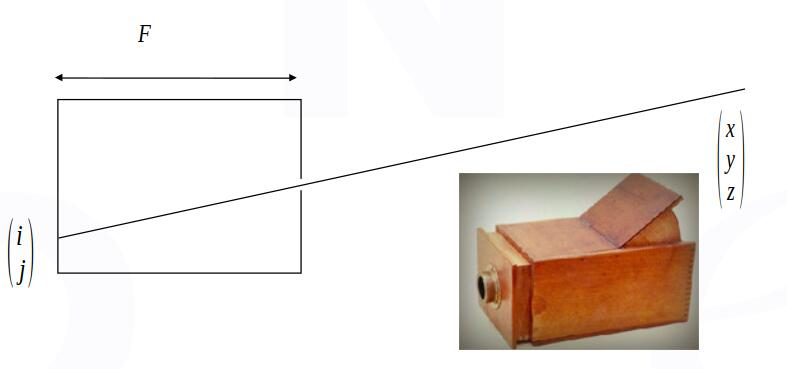
\includegraphics[width=12cm]{Methods/Images/CameraObscura.jpg}\caption{Camera osbcura : schema and a real object}
	\label{fig:CameraObscura}
\end{figure}


We begin by the description of very simple object, but which is really a the origin of
the photography and, in some way, is the simplest possible camera  :  the camera obscura.
Basically it can be described as a box with a hole, at the entrance of the box we have
a the hole that let the light in, and at the bottom of the box we have the film of
the camera. 

Figure~\ref{fig:CameraObscura} presents a real camera and a basic schema showing
the construction of the image :  to compute the image of a point $P^c=x^c,y^c,z^c$ of the real scene
we juts have to trace the line starting from $P^c$, going throw the hole and take its intersection $q=i,j$
with the image plane.


%-----------------------------------------------------
\subsection{Setting equations}

To compute a mathematical relation between $x^c,y^c,z^c$ and $i,j$ we will introduce several hypothesis 
and notation illustrated by figure~\ref{fig:Camera3DNote} :

\begin{figure}
\centering
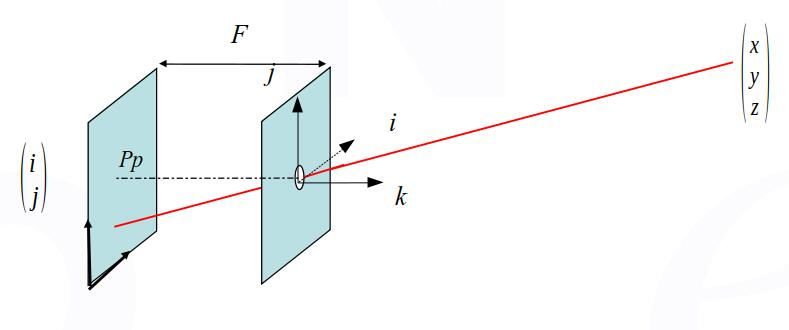
\includegraphics[width=12cm]{Methods/Images/Camera3D.jpg}\caption{Notation for camera relation}
	\label{fig:Camera3DNote}
\end{figure}

\begin{itemize}
	\item for $x,y,z$ we consider a local $3d$ repair $(O,\vec{i},\vec{j},\vec{k})$  where $O$ is the entrance hole,
              $\vec{i},\vec{j}$ belongs to the image plane and $\vec{k}$ is orthogonal to  $\vec{i}$ and $\vec{j}$;

	\item for $i,j$ we consider a image repair originated at one corner $c$ of the box;

	\item we note $P^p$ (principal point)  the intersection of axe $O\vec{k}$  with the image plane,
	      and $F$ (focal length) the distance between $PP$ and $O$.

        \item we note $Q_3$  the $3d$ point corresponding to $q$.

\end{itemize}

To compute coordinates of $Q_3$ we can use chasles relation as indicated in equation~\ref{PC:Chasles} :

\begin{equation}
	\overrightarrow{OQ_3} =  \overrightarrow{O P^p} + \overrightarrow{P^p c} +  \overrightarrow{c Q_3}
	 =     \begin{pmatrix} 0\\0\\-F \end{pmatrix}
             + \begin{pmatrix} -P^p_x\\-P^p_y\\0 \end{pmatrix}
             + \begin{pmatrix} i\\j\\0 \end{pmatrix}
	 =     \begin{pmatrix} i-P^p_x\\j-P^p_y\\-F \end{pmatrix}
	\label{PC:Chasles}
\end{equation}

Now remind that light having a straight walk, the $3$ point $Q_3$, $0$ and $P^c$ must be aligned,
which can be wrotten by equation~\ref{PC:Alignment} :

\begin{equation}
	\exists \lambda : 
	\begin{pmatrix} i-P^p_x\\j-P^p_y\\-F \end{pmatrix} 
      = \lambda   \begin{pmatrix} x^c\\y^c\\z^c \end{pmatrix}
		\label{PC:Alignment}
\end{equation}

By a quotient  we can elimimnate $\lambda$ in~\ref{PC:Alignment} and obtain :


\begin{equation}
	i = P^p_x -F \frac{x^c}{z^c}  \; ; \;
	j = P^p_y -F \frac{y^c}{z^c}  
	\label{PC:FormulaImaIntr1}
\end{equation}

%-----------------------------------------------------
\subsection{Image formula, local}

The usage is to modiy the equation~\ref{PC:FormulaImaIntr1} by changing the sign of $F$;
this comes to consider a camera model ,
 not physically feasible and slightly different from the camera obscura,  
where the image plane is before the whole instead of behing, and that
is illustrated by figure~\ref{fig:PcInvCam}.  

\begin{figure}
\centering
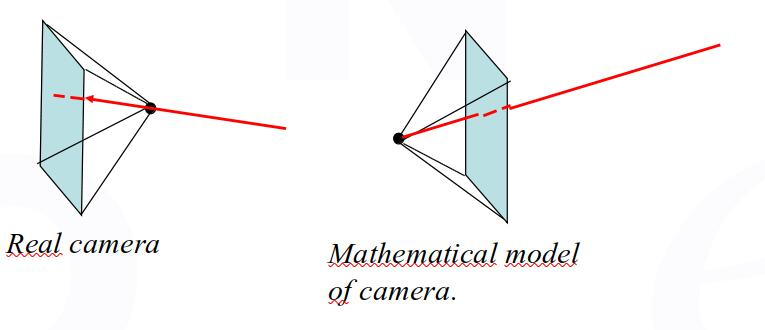
\includegraphics[width=12cm]{Methods/Images/InvCamera.jpg}
	\caption{Camera model : physically based one (left) and used one (right)}
	\label{fig:PcInvCam}
\end{figure}

Finally we will use equation~\ref{PC:FormulaImaIntr2} to formulate the relation between
local ground coordinates $P^c$  and image coordinate for this basic camera :

\begin{equation}
	i = P^p_x +F \frac{x^c}{z^c}  \; ; \;
	j = P^p_y +F \frac{y^c}{z^c}  
	\label{PC:FormulaImaIntr2}
\end{equation}

Setting the canonical projection $\pi$:

\begin{equation}
	  \pi \begin{pmatrix} x^c \\ y^c \\ z^c \end{pmatrix} 
           =  \begin{pmatrix} \frac{x^c}{z^c} \\  \frac{x^c}{z^c}  \end{pmatrix} 
\end{equation}

and the intrinsic calibration $ \mathcal{I}_0$ :

\begin{equation}
	   \mathcal{I}_0  \begin{pmatrix} u \\  v  \end{pmatrix} 
        =  P^p + F  \begin{pmatrix} u \\  v  \end{pmatrix}
\end{equation}

we will write :

\begin{equation}
	q  =   \mathcal{I}_0 (\pi (P^c))
\end{equation}


%-----------------------------------------------------
\subsection{Image formula, global}

Generally need to write the coordinate of $q$ as a function of the global coordinate $P$ or a point.
For this we just have to write $P^c$ as a function of $P$, we use $C$ the center of the camera, and
$R$ its orientation :

\begin{equation}
	P =  C+ R *P_c
\end{equation}

Which give the image formula :
\begin{equation}
	q  =   \mathcal{I}_0 (\pi (^t R (P - C))) \label{FormImage0}
\end{equation}

This formula will follow us for a long time. The main thing that will evolve is $\mathcal{I}_0$
that will become more complicated to take into account lenses used in real camera.


%-----------------------------------------------------
\subsection{A remark on repair orientation}

\begin{figure}
\centering
	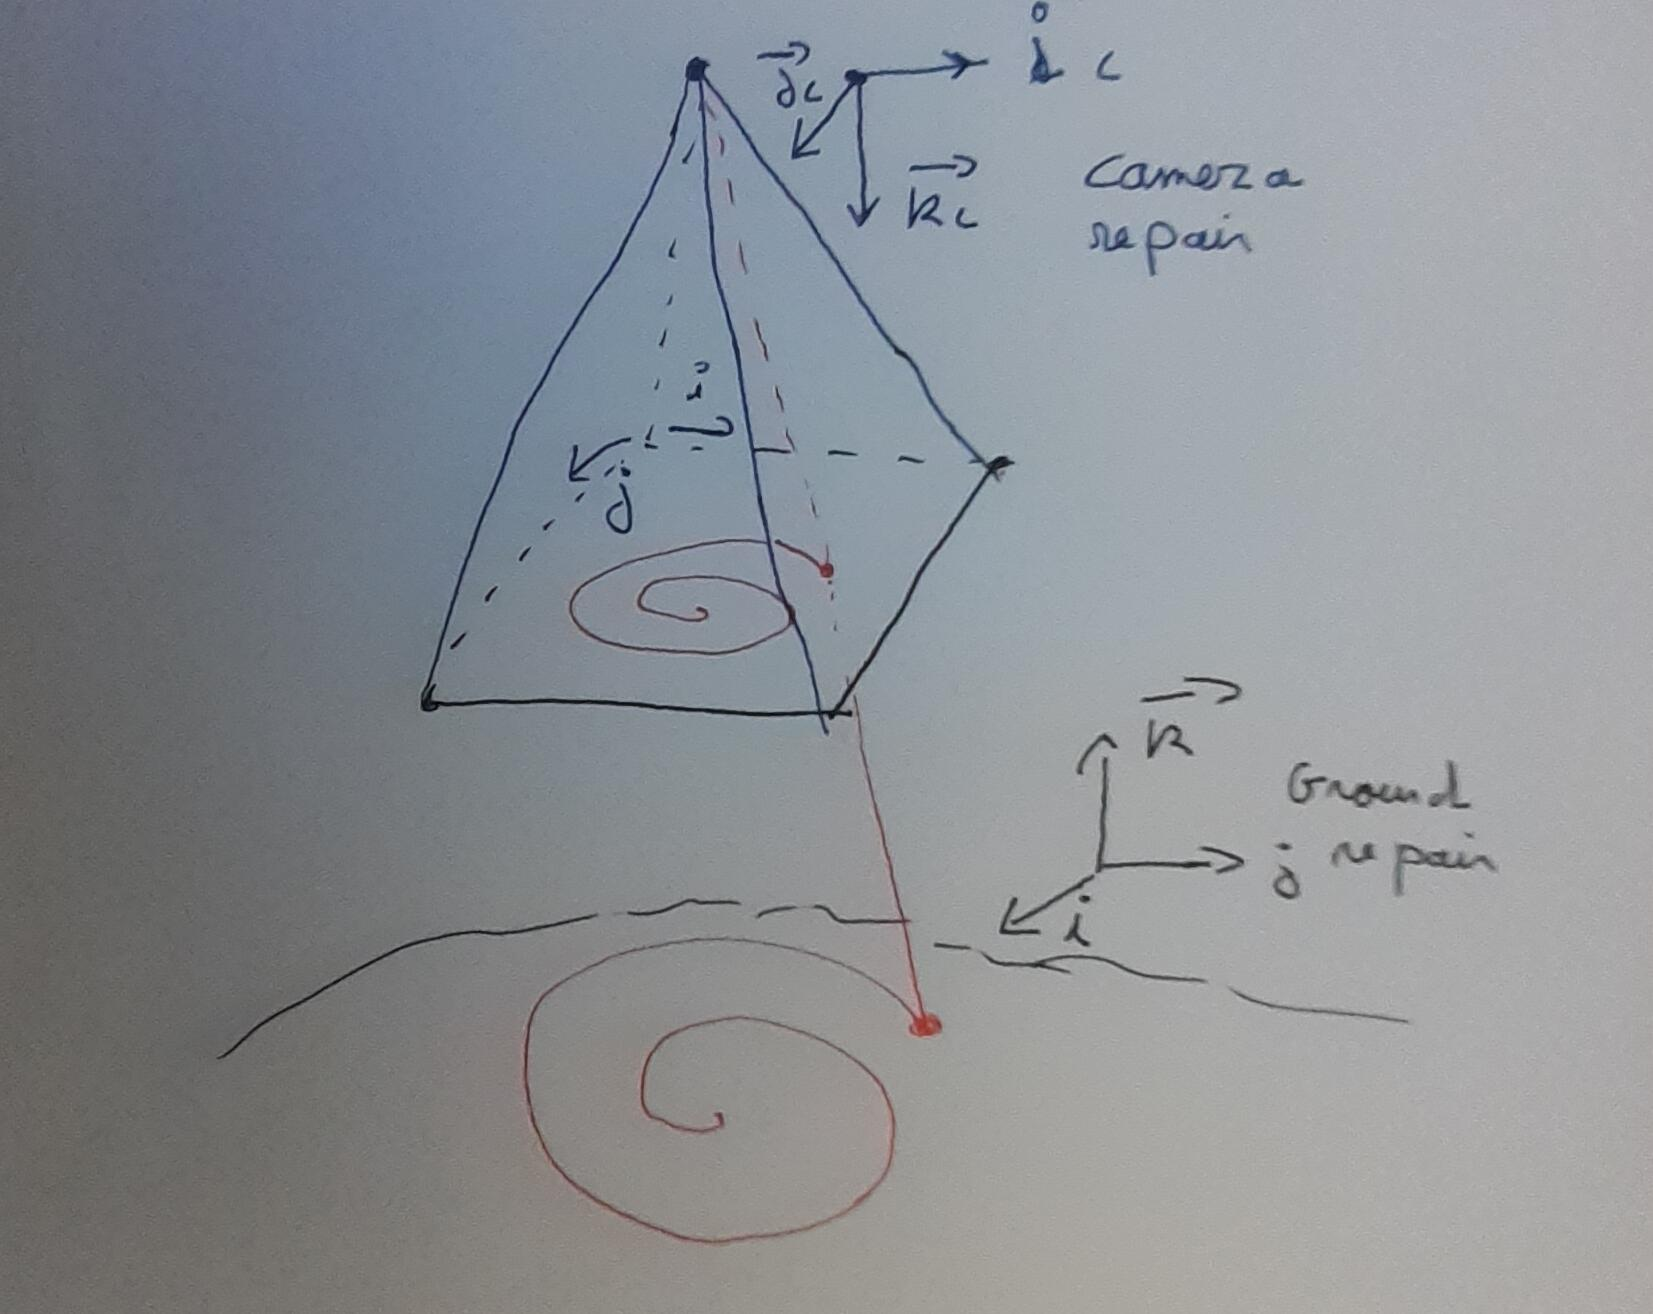
\includegraphics[width=12cm]{Methods/Images/RepairCam.jpg}
	\caption{Camera model : physically based one (left) and used one (right)}
	\label{fig:FormIm}
\end{figure}

%-----------------------------------------------------
%-----------------------------------------------------
%-----------------------------------------------------

\section{Radial modelisation}


%-----------------------------------------------------
%-----------------------------------------------------
%-----------------------------------------------------

\section{Decentric distorsion}


%-----------------------------------------------------
%-----------------------------------------------------
%-----------------------------------------------------

\section{General model}

\subsection{Fish eye model}
\subsection{$360$ camera}
\subsection{Assemblage camera}

%-----------------------------------------------------
%-----------------------------------------------------
%-----------------------------------------------------

\section{Planary inclinaison}




